%% ----------------------------------------------------------------
%% Thesis.tex -- MAIN FILE (the one that you compile with LaTeX)
%% ---------------------------------------------------------------- 

% Set up the document
\documentclass[a4paper, 11pt, oneside]{Thesis}  % Use the "Thesis" style, based on the ECS Thesis style by Steve Gunn
\graphicspath{Figures/}  % Location of the graphics files (set up for graphics to be in PDF format)

% Include any extra LaTeX packages required
\usepackage[square, numbers, comma, sort&compress]{natbib}  % Use the "Natbib" style for the references in the Bibliography
\usepackage{verbatim}  % Needed for the "comment" environment to make LaTeX comments
\usepackage{vector}  % Allows "\bvec{}" and "\buvec{}" for "blackboard" style bold vectors in maths
\hypersetup{urlcolor=blue, colorlinks=true}  % Colours hyperlinks in blue, but this can be distracting if there are many links.

\usepackage{eurosym} % Euro symbol

%% ----------------------------------------------------------------
\begin{document}
\frontmatter      % Begin Roman style (i, ii, iii, iv...) page numbering

% Set up the Title Page
\title  {\ThesisName{}}
\authors  {\texorpdfstring
            {\href{alu0100775846@ull.edu.es}{\AuthorName{}}}
            {José ...}
            }
\addresses  {\groupname\\\deptname\\\univname}  % Do not change this here, instead these must be set in the "Thesis.cls" file, please look through it instead
\date       {\today}
\subject    {}
\keywords   {PLN}

\maketitle
%% ----------------------------------------------------------------

\setstretch{1.3}  % It is better to have smaller font and larger line spacing than the other way round

% Define the page headers using the FancyHdr package and set up for one-sided printing
\fancyhead{}  % Clears all page headers and footers
\rhead{\thepage}  % Sets the right side header to show the page number
\lhead{}  % Clears the left side page header

\pagestyle{fancy}  % Finally, use the "fancy" page style to implement the FancyHdr headers

\pagestyle{empty}  % Page style needs to be empty for this page

\btypeout{Licencia}
\null\vfil
\vskip 60pt
\begin{center}{
\begin{figure}[!ht]
  \centering
    
\includegraphics[]{Images/cc}
\end{figure}
Esta obra está bajo una licencia de Creative
Commons Reconocimiento 4.0 Internacional.

This work is licensed under a Creative Commons Attribution-ShareAlike 4.0 International License.
}\end{center}
\vfil\null
\cleardoublepage

\clearpage  % CC ended, start a new page % Creative Commons

%% ----------------------------------------------------------------
% Declaration Page required for the Thesis, your institution may give you a different text to place here
%\Declaration{

\addtocontents{toc}{\vspace{1em}}  % Add a gap in the Contents, for aesthetics

Dña. Coromoto León Hernández, con N.I.F 78.605.216-W, profesora Titular de Universidad adscrita al Departamento de Ingeniería Informática y de Sistemas, como tutora

%\textbf{CERTIFICA}
\textbf{C E R T I F I C A}

\begin{itemize} 
\item[] Que la presente memoria titulada:
 
\item[] \say{\textit{\ThesisName{}}}
 
\item[] ha sido realizada bajo su dirección por D. \textbf{\AuthorName{}},
 
\item[] con N.I.F. 54.112.122-E.
 
\item[] Y para que así conste, en cumplimiento de la legislación vigente y a los efectos oportunos firma la presente en La Laguna a 5 de septiembre de 2016.
\\
\end{itemize}


 
%Signed:\\
%\rule[1em]{25em}{0.5pt}  % This prints a line for the signature
 
%Date:\\
%\rule[1em]{25em}{0.5pt}  % This prints a line to write the date
%}
\clearpage  % Declaration ended, now start a new page % Declaration Page

%% ----------------------------------------------------------------
% The "Funny Quote Page"
\pagestyle{empty}  % No headers or footers for the following pages

\null\vfill
% Now comes the "Funny Quote", written in italics
\textit{``If you talk to a man in a language he understands, it will go to his head. If you talk to him in his own language, it will go to his heart.''}

\begin{flushright}
Nelson Mandela
\end{flushright}

\vfill\vfill\vfill\vfill\vfill\vfill\null
\clearpage  % Funny Quote page ended, start a new page
%% ---------------------------------------------------------------- % Funny Quote

% The Abstract Page
\addtotoc{Abstract}  % Add the "Abstract" page entry to the Contents
%\abstract{
\addtocontents{toc}{\vspace{1em}}  % Add a gap in the Contents, for aesthetics

\bigskip
%\center{\huge{\textit{Abstract}} \par}
\begin{center}
\huge{\textit{Abstract}} \par
\end{center}

%The aim of this work is to study the currently available tools for Natural Language Processing that might be applied in study cases for the Spanish language, as most of these tools nowadays focus on the English language.

The aim of this work is the development of a study case in Spanish in which Natural Language Processing techniques are applied, to observe the effectiveness of the NLP tools available for this language.

The study case chosen for this work is the classification of the Final Degree Projects made avaliable to the public in the Institutional Repository of the University of La Laguna.
%}
\vskip 40pt
\textbf{Keywords:} \textit{NLP, Natural Language Processing, NLTK, Natural Language Toolkit, Python, CasperJS, JavaScript}

%\bigskip
\clearpage
\addtotoc{Resumen}
%\center{\huge{\textit{Resumen}} \par}
\begin{center}
\huge{\textit{Resumen}} \par
\end{center}

%La finalidad de este trabajo es el estudio de las herramientas actualmente disponibles para el Procesamiento del Lenguaje Natural que puedan ser aplicadas a casos de estudio para el idioma español, dado que la mayoría de estas herramientas hoy en día se centran en el inglés.

La finalidad de este trabajo es el desarrollo de un caso de estudio en lenguaje español sobre el cual aplicar técnicas de Procesamiento del Lenguaje Natural, para constatar la eficacia de las herramientas PLN disponibles para este idioma.

El caso de estudio escogido para desarrollar en este trabajo fue la clasificación de los Trabajos de Fin de Grado puestos a disposición del público en el Repositorio Institucional de la Universidad de La Laguna.

\vskip 40pt
\textbf{Palabras clave:} \textit{PLN, Procesamiento del Lenguaje Natural, NLTK, Natural Language Toolkit, Python, CasperJS, JavaScript}
%}

\clearpage  % Abstract ended, start a new page
%% ---------------------------------------------------------------- % Abstract

\setstretch{1.3}  % Reset the line-spacing to 1.3 for body text (if it has changed)

% The Acknowledgements page, for thanking everyone
\acknowledgements{
\addtocontents{toc}{\vspace{1em}}  % Add a gap in the Contents, for aesthetics

A mi tutora, Coromoto León Hernández, por su dirección, optimismo y apoyo incondicional a la hora de encaminar el proyecto.

Al personal docente de la facultad de Informática, por su labor educativa.

A mis amigos y compañeros de la facultad, por el apoyo recibido.

A mi familia, y mis padres, por su paciencia, cariño y por hacer posible mi educación.
}
\clearpage  % End of the Acknowledgements
%% ----------------------------------------------------------------
 % Acknowledgements

\pagestyle{fancy}  %The page style headers have been "empty" all this time, now use the "fancy" headers as defined before to bring them back


%% ----------------------------------------------------------------
\lhead{\emph{Contents}}  % Set the left side page header to "Contents"
\tableofcontents  % Write out the Table of Contents

%% ----------------------------------------------------------------
\lhead{\emph{Índice de figuras}}  % Set the left side page header to "List of Figures"
\listoffigures  % Write out the List of Figures

%% ----------------------------------------------------------------
\btypeout{Lista de listados}
\addtotoc{Lista de listados}
\lhead{\emph{Lista de listados}}  % Set the left side page header to "List of Listings"
\lstlistoflistings  % Write out the List of Listings

%% ----------------------------------------------------------------

\lhead{\emph{Índice de cuadros}}  % Set the left side page header to "List of Tables"
\listoftables  % Write out the List of Tables

%%% ----------------------------------------------------------------
% Begin the Dedication page

\setstretch{1.3}  % Return the line spacing back to 1.3

\pagestyle{empty}  % Page style needs to be empty for this page
\dedicatory{A mi familia}

\addtocontents{toc}{\vspace{2em}}  % Add a gap in the Contents, for aesthetics
 % Dedication

%% ----------------------------------------------------------------
\mainmatter	  % Begin normal, numeric (1,2,3...) page numbering
\pagestyle{fancy}  % Return the page headers back to the "fancy" style

% Include the chapters of the thesis, as separate files
% Just uncomment the lines as you write the chapters

% TODO correct lheads, they show up improperly
% maybe if I put lheads inside chaps, or end chaps
% with \newpage...

\lhead{\emph{\ChapterOne{}}}
\chaptermark{\emph{\ChapterOne{}}}
\chapter{\ChapterOne{}}
\lhead{\emph{\ChapterOne{}}}

\lhead{\emph{\ChapterOne{}}}
El Procesamiento del Lenguaje Natural (PLN) es una disciplina de la Computación que concierne al tratamiento de información desestructurada, presentada en texto o audio y expresada mediante Lenguaje Natural.
%
Se entiende por lenguaje natural cualquier lenguaje utilizado para la comunicación humana en el día a día, en contraposición a un lenguaje artificial establecido, como por ejemplo los lenguajes de programación.
%
Es un área de interés para el campo de la Interacción Persona-Computador (\textit{Human-Computer Interaction}), así como los de Aprendizaje Automático (\textit{Machine Learning}) e Inteligencia Artificial (\textit{Artificial Intelligence}).

La necesidad del Procesamiento del Lenguaje Natural es aparente en los sistemas de Interacción Persona-Computador, dado que en este campo se busca el diseño de interfaces cómodas y funcionales para los usuarios humanos a la hora de utilizar ordenadores, ya sean tradicionales, portátiles, móviles, etc.
%
El Procesamiento del Lenguaje Natural se posiciona como una capacidad deseable en los ordenadores, para permitir la comunicación natural entre el usuario y el ordenador, y aumentar tanto la comodidad y conveniencia como las posibilidades de una interacción exitosa.

En cuanto al campo del Aprendizaje Automático, no sólo nos referimos al hecho de que éste campo es necesario para el desarrollo de técnicas PLN, sino que el campo del Procesamiento del Lenguaje Natural a su vez puede ser útil para el Aprendizaje Automático en uno de sus mayores problemas.
%
Uno de los principales cuellos de botella hoy en día a la hora de la construcción de sistemas de Aprendizaje Automático es la insuficiente cantidad de datos estructurados. El Procesamiento del Lenguaje Natural permite la conversión de los datos desestructurados en lenguaje natural en datos estructurados con los cuales un sistema informático pueda aprender.

Sólo por esto es por extensión de importancia para el campo de la Inteligencia Artificial, ya que los recientes avances en dicho campo se basan en el Aprendizaje Automático y por tanto se beneficia de las mejoras que el PLN pueda aportar al mismo.
%
No es necesario concretar la importancia del PLN en el campo de la Inteligencia Artificial, ya que las primeras definiciones de una máquina inteligente (el Test de Turing) presuponen una capacidad de procesamiento e interpretación del lenguaje humano.

En otros campos de la ciencia se ha hablado extensamente de la importancia del lenguaje como factor decisivo para la producción de inteligencia tal y como la definimos, tanto así que existe una rama de la ciencia, la neurolinguística, centrada exclusivamente en el estudio de este fenómeno.

---

Para facilitar la fluidez en la lectura del documento, se hace uso de términos y abreviaturas que pueden ser propias del área de conocimientos a tratar o simplemente sean de nueva introducción, por lo que se proporciona un glosario como apéndice auxiliar con el fin de esclarecer su significado.

En el siguiente apartado, se hace una revisión de las áreas temáticas y herramientas en las que se subdivide el campo del Procesamiento del Lenguaje Natural. El resto del Capítulo 1 está dedicado a las herramientas consideradas para la realización del caso de estudio.

\lhead{\emph{\ChapterOne{}}}
\section{Estado del arte}

El estado actual del campo tiene numerosas áreas temáticas que se pueden subclasificar en herramientas conceptuales y aplicaciones. Una lista extensa de éstas se define en el número 56 de la Revista de Procesamiento de Lenguaje Natural \cite{sepln-56}:
        
\textbf{Modelos lingüísticos, matemáticos y psicolingüísticos del lenguaje}, refiriéndonos al PLN enfocado como un sistema de reglas.

\textbf{Lingüística de corpus}, metodología en la que se estudia el lenguaje a través de ejemplos de textos reales producidos en el mundo real.

\textbf{Desarrollo de recursos y herramientas lingüísticas}, en aquéllos trabajos que expanden las herramientas PLN disponibles para su futuro uso.

\textbf{Gramáticas y formalismos para el análisis morfológico y sintáctico}, refiriéndonos al PLN enfocado como un sistema de reglas lógicas aplicado al análisis morfosintáctico.

\textbf{Semántica, pragmática y discurso}. El estudio tradicional del lenguaje natural para cada idioma por parte de lingüistas nos permite abstraer las reglas para su uso y comprensión.

\textbf{Lexicografía y terminología computacional}, que busca una sistemática colección y explicación de todas las palabras (o más estrictamente, unidades léxicas) de un lenguaje. 

\textbf{Resolución de la ambigüedad léxica}, siendo un ejemplo la determinación del sustantivo concreto dada una referencia indirecta.

\textbf{Aprendizaje automático en PLN}, es decir la aplicación de algoritmos de aprendizaje no supervisado para sistemas de esta índole.

\textbf{Generación textual monolingüe y multilingüe}. Esto es, la expresión en lenguaje natural de información estructurada, permitiendo a un ordenador generar a tiempo real respuestas más accesibles a un usuario.

\textbf{Traducción automática}, refiriéndonos a sistemas capaces de realizar la traducción de textos naturales a otro lenguaje natural con poca o nula supervisión humana.

\textbf{Reconocimiento y síntesis del habla}, atendiendo a problemática como la determinación de palabras homófonas a través del contexto.

\textbf{Extracción y recuperación de información monolingüe, multilingüe y multimodal}, en la que se aprovecha información multimedia recibida a tiempo real para analizar la intención del emisor.

\textbf{Sistemas de búsqueda de respuestas}, alternativas a los históricos sistemas expertos, en los que se pretende responder a preguntas del usuario sobre un ámbito reducido.

%\textbf{Análisis automático del contenido textual}.

\textbf{Resumen automático}, por el cual obtenemos el resumen de un texto intentando conservar la información relevante.

%\textbf{PLN para la generación de recursos educativos}.

\textbf{PLN para lenguas con recursos limitados}, como es el caso de lenguas indígenas o autóctonas.

\textbf{Aplicaciones industriales del PLN}, entre las más importantes la generación de información para la toma de decisiones en empresas, o Inteligencia Empresarial (\textit{Business Intelligence}).

\textbf{Sistemas de diálogo}, sistemas que se comunican con el usuario utilizando lenguaje natural, de manera similar a mantener una conversación. 

\textbf{Análisis de sentimientos y opiniones}, actualmente un área del PLN con gran popularidad y que puede considerarse como una de sus aplicaciones industriales de mayor interés.

\textbf{Minería de texto}, el procesamiento estadístico de grandes cantidades de texto con la intención de extraer información de alta calidad.

%\textbf{Evaluación de sistemas de PLN}.

\textbf{Implicación textual y paráfrasis}, con la que podemos visualizar información textual de diversas maneras, así como conocer las enunciaciones que se derivan de ellas.

Se tuvieron en cuenta estas áreas temáticas a la hora de decidir el enfoque que tendría el trabajo, tomando en cuenta variables como factibilidad, tiempo disponible y utilidad, entre otras.



\section{Ámbito del problema}

Se decidió realizar un trabajo sobre Procesamiento de Lenguaje Natural, siendo este el primer punto acordado antes de proceder a la definición del problema a tratar para la realización del trabajo.

\section{Definición del problema}

El caso de estudio escogido para este trabajo puede ser subdividido en dos problemas: el primero es la obtención del texto a clasificar, ya sea desde un archivo de texto en local o a través de Internet.

El segundo problema es el más importante y el cual es objetivo principal de este trabajo: el procesamiento del texto una vez obtenido.

Se ha decidido presentar las secciones de manera cronológicamente equivalente a la que se produce en cualquier problema de Procesamiento de Lenguaje Natural.

%% TODO : Does this go here?

%\subsection{Datos de trabajo}

\subsection{Obtención del texto}

Hoy en día existen muchas fuentes de las cuales obtener texto a la hora de realizar procesamiento de texto: se puede obtener de Internet, puede ser creado o incluso puede obtenerse de un medio físico como pueden ser los libros o la voz de un usuario.

La obtención del texto a procesar puede realizarse de muchas maneras, existiendo varias opciones para cada fuente de texto que se puede presentar. 

En el caso de Internet, existen tanto librerías para lenguajes de programación como programas dedicados a la extracción de texto. Normalmente funcionan de manera similar a un navegador de Internet, utilizando el protocolo HTTP para enviar peticiones a servidores web y recibir contenidos de las páginas web, que luego son desglosados mediante \textit{parsers} para obtener los datos deseados.

En nuestro caso, el objetivo es la clasificación de los Trabajos de Fin de Grado. El Repositorio Institucional de la Universidad de La Laguna \cite{riull} es un Servicio Web que contiene una gran cantidad de documentos relacionados con la actividad docente de la Universidad, entre ellos los Trabajos de Fin de Grado.

\subsection{Procesamiento del texto}

El procesamiento de texto es la parte del problema que toma una mayor importancia, ya que es la más complicada y objeto de este trabajo.

Para nuestro caso de estudio, nos concentramos en un subproblema del campo; la clasificación de textos. La clasificación de textos es una de las de mayor relevancia actual.

\lhead{\emph{\ChapterOne{}}}
El estudio previo de las opciones a considerar a la hora escoger las herramientas para realizar el proyecto ha ocupado una gran parte del tiempo dedicado.

Esto es en parte debido a la gran cantidad de herramientas disponibles para la tarea a realizar: existen decenas de herramientas para el Procesamiento del Lenguaje Natural, y cientos para la extracción de texto a partir de fuentes en Internet.

Para realizar el trabajo se han considerado varias herramientas, teniendo en cuenta puntos como la facilidad de uso, la adaptabilidad de la herramienta, su capacidad de procesamiento, las posibilidades de ser utilizada con entradas de texto en español, etc.

\section{Herramientas de PLN}

Se consideró un número de herramientas para el Procesamiento del Lenguaje Natural, las cuales fueron evaluadas según las ventajas y desventajas que proporcionarían al desarrollo del proyecto teniendo en cuenta los objetivos que se deseaban alcanzar.

La herramienta utilizada en este caso es la biblioteca NLTK (\textit{Natural Language Toolkit}) desarrollada en el lenguaje de programación Python, pero es necesario conocer las decisiones que llevaron a esta conclusión.

A continuación se muestran las herramientas consideradas para el Procesamiento del Lenguaje Natural en la realización de este trabajo.

\subsection{Stanford CoreNLP}

Se trata de una herramienta de Procesamiento de Lenguaje Natural implementada en Java por la Universidad de Stanford \cite{stanford-corenlp-paper}.
%
%(Ha sido implementada en Java, y la ...entrega... actual requiere Java 1.8+).
%
Fue una de las herramientas de mayor importancia a considerar, debido a la familiaridad que se tenía con la metodología de trabajo a la hora de utilizarlo.
%
Actualmente cuentan con modelos lingüísticos para el chino, inglés, francés, alemán, y español, el idioma objetivo de este trabajo.
%
Una de las principales ventajas de esta herramienta es su implementación en Java, un lenguaje de más bajo nivel que Python o Ruby, lo que le proporciona una mayor capacidad de cómputo de datos.

\subsection{Apache Lucene y Solr}

Una de las grandes ventajas del sistema Solr es que posee una API (\textit{Application Programming Interface}) flexible con la que se puede interactuar mediante los lenguajes de programación Ruby y Python, así como también es posible comunicarnos mediante el paso de mensajes JSON (JavaScript Object Notation), de manera similar a muchas arquitecturas servidor/cliente en la red \cite{apache-lucene}.

\subsection{Apache OpenNLP}

Esta herramienta utiliza una aproximación diferente a la que usa el Stanford CoreNLP.
%
Se trata de un sistema desarrollado en Java, que permite ser utilizado como una biblioteca Java. Además de esto, posee una interfaz de programación en línea (\textit{scripting}) que puede también usarse mediante la línea de comandos \cite{apache-open-nlp}.
%
A pesar de encontrarse algo desfasada en comparación con el resto de opciones, permanece como una opción robusta y rápida de implementar.

%\subsection{Apache UIMA}

%Se observó otra herramienta Apache para el Procesamiento de Lenguaje Natural...

%\subsection{FreeLing}
%asd

\subsection{GATE}

El GATE (\textit{General Architecture for Text Engineering}) es un sistema de software libre con una gran capacidad de procesamiento de texto \cite{gate}.
%
Fue desarrollado inicialmente por un equipo base de 16 programadores \cite{gate-about}, empezando en 1995 como parte de un proyecto del EPSRC (Engineering and Physical Sciences Research Council), una organización basada en el Reino Unido con el objetivo de financiar la investigación científica en el país.
%
Dado el largo tiempo que lleva esta herramienta en desarrollo, que abarca más de dos décadas, cuenta con un amplio abanico de funcionalidades de procesamiento de texto.

\subsection{NLTK, Natural Language Toolkit}

El NLTK (\textit{Natural Language Toolkit}) es una biblioteca de Procesamiento de Lenguaje Natural que utiliza el lenguaje de programación Python \cite{nltk-book}.
%
NLTK es software libre, lo que permite a estudiantes y al personal académico realizar estudios con la herramienta sin necesidad de realizar una inversión económica.
%
Esta herramienta es también de código abierto, lo que lo hace ideal para expandir sus funcionalidades en caso de necesitarlo.
%
El hecho de estar implementada como una biblioteca Python reduce la curva de aprendizaje, y la acerca al mundo académico, cuya mayor parte de integrantes se encuentra familiarizado con este lenguaje de programación.

\label{chosen-nlp-tool}
\section{Herramienta de PLN elegida}

Una razón para la elección de NLTK como herramienta es el gran soporte que tiene, debido a las dimensiones de su comunidad de usuarios. Es una de las herramientas de Procesamiento de Lenguaje Natural de mayor aceptación en el ámbito científico.

Otra razón importante es el apoyo que proporciona el libro \textit{Natural Language Processing with Python}\cite{nltk-book}. Este libro tiene por autores a los creadores del NLTK, haciéndolo idóneo para comprender y utilizar todas las funcionalidades que aporta esta biblioteca.

\section{Lenguaje de programación escogido}

El código de las herramientas de Procesamiento de Lenguaje Natural desarrolladas en Java y C++ es compilado a un código máquina de bajo nivel, lo que le confiere una mayor rapidez de cómputo.

Ésta amplia capacidad de procesamiento en comparación a herramientas para Python o Ruby es aprovechable ya sea en aumentar la cantidad de datos a procesar o reducir el tiempo que lleva el procesamiento de los mismos.

Sin embargo, el que una herramienta esté diseñada para un lenguaje de éstas características tiene como consecuencia la reducción de flexibilidad inmediata de la herramienta, ya que el desarrollo de software en los lenguajes fuertemente tipados conlleva una mayor cantidad de tiempo a la hora de especificar la relación, jerarquía y tipado de los datos, con el fin de aprovechar el aumento en velocidad que ofrecen.

Es por esta razón que se optó por lenguajes de guiones (\textit{scripting}), como Python o Ruby, que sin perder generalidad en cuanto a la resolución de problemas, y a pesar de tener una velocidad de cómputo más reducida, permiten el desarrollo de soluciones adaptadas a los problemas que surgen con una mayor flexibilidad y rapidez, ofreciendo además una mayor cantidad de funcionalidad estándar para el procesamiento de texto.

Se decidió utilizar Python para complementar la elección de herramienta de PLN que se hizo, en este caso la biblioteca NLTK para Python, como se mencionó anteriormente (\ref{chosen-nlp-tool}).


---

A continuación, en el Capítulo 2, se expone la problemática concreta del caso de estudio así como las soluciones implementadas con las herramientas escogidas. El Capítulo 3 expone los resultados alcanzados y realiza una comparativa, mientras que el Capítulo 4 extrae conclusiones sobre el trabajo realizado, y plantea futuras líneas de trabajo. Finalmente, el Capítulo 5 desglosa los recursos utilizados en la elaboración de este proyecto. % Introduction

\lhead{\emph{\ChapterTwo{}}}
\chaptermark{\emph{\ChapterTwo{}}}
\chapter{\ChapterTwo{}} \label{amigo}
\lhead{\emph{\ChapterTwo{}}}

En este capítulo procederemos a explicar el caso de estudio escogido para el desarrollo del trabajo, así como la problemática asociada y las soluciones implementadas para el desarrollo de la misma. En primer lugar hablaermos del 

\section{Descripción del caso de estudio}

El caso de estudio escogido consiste en la clasificación de los Trabajos de Fin de Grado (TFGs) que se encuentran en el Repositorio Institucional de la ULL, partiendo de la información que se puede recabar sobre los mismos.
%
El objetivo de este caso de estudio es el de obtener un sistema de clasificación de TFGs que pueda servir como suplemento a la hora de asignar un área temática a un TFG cuando éste es inscrito a la plataforma.

\section{Opciones de clasificación}

La clasificación de textos es un subproblema del campo del Procesamiento del Lenguaje Natural, entre muchos otros como aquéllos discutidos en el capítulo anterior (\ref{amigo}).
%
Fue escogido debido a la facilidad y rapidez de su implementación con las herramientas disponibles a día de hoy, entre ellas el NLTK.
%
Existen varias formas de realizar la clasificación de un texto, todas claramente atendiendo a las características del mismo, pero utilizando diferentes enfoques.
%
En las siguientes secciones pasamos a describir los enfoques más utilizados para ello.

\subsection{Enfoques estadísticos}

Esta clase de enfoques hacen uso de las técnicas de Aprendizaje Automático, que hoy en día son las que gozan de mayor aceptación y crecimiento.
%
Utilizan técnicas estadísticas para realizar estimaciones sobre un conjunto de datos del que se desconoce una o varias características, y se procede a asignar
%
El éxito de este tipo de técnicas se basa en las características que sean detectadas y seleccionadas como relevantes para el problema de clasificación que se tenga.

\begin{minipage}{\linewidth}
\textit{Tomemos como ejemplo un hipotético estudio sobre los hábitos alimenticios de un grupo de animales.
El color del pelaje de un animal no es relevante a la hora de inferir su dieta, pero en cambio la clase de dentadura que posea sí lo es. Por tanto, en este caso se deberá ignorar el color del pelaje pero tomar en cuenta el tipo de dentadura de los animales.}
\end{minipage}

%Por tanto, es 

Para los casos de aprendizaje supervisado, existen elementos ya clasificados de manera correcta, ya sea por parte de otro programa o de manera manual. Estos elementos son utilizados para conformar un subconjunto de entrenamiento.

En estos casos de aprendizaje supervisado, es importante cuidarse de no sobreajustar el clasificador a la clasificación de los problemas de entrada. 
%
El problema del sobreajuste es un problema difícil de resolver objetivamente, y suele manejarse mejor cuando se tiene un cierto nivel de experiencia en tratar con él.

En el caso del aprendizaje no supervisado, no se poseen de datos de entrenamiento, por lo que normalmente recae sobre el algoritmo la diferenciación de los elementos en diferentes clases \say{a posteriori}, es decir, clases que no habían sido definidas antes de la tarea de clasificación.

%Este método puede brindar nuevas maneras de...

%Uno de los problemas que tiene esta clase de enfoque es que muchas veces no proporciona un modelo claro, con algunas excepciones, de la lógica utilizada para clasificar los textos.

%Las excepciones a la regla son los árboles de clasificación, que pueden ser utilizados una vez se conoce la estructura del problema.
%Si se desconoce la estructura del problema pero en cambio se tienen datos etiquetados, pueden ser generados mediante técnicas de Aprendizaje Automático.

\subsection{Naive Bayes}

Los clasificadores de Bayes ingenuos (\textit{Naive Bayes classifiers}) son clasificadores utilizados ampliamente en la actualidad para problemas de clasificación de textos, tanto en ámbitos académicos como industriales.

Los caracteriza una gran simplicidad, que conlleva la ventaja de que son de fácil comprensión y por tanto de fácil uso.

A pesar de esta simplicidad, los clasificadores de Bayes ingenuos son bastante eficaces y tienen una gran cantidad de aplicaciones prácticas.

Los clasificadores de Bayes ingenuos se basan en un modelo probabilístico, el Teorema de Bayes.

\begin{equation}\label{eq:bayes}
    p(C_k|x) = \frac{p(C_k)p(x|C_k)}{p(x)}
\end{equation}

Según este teorema, la probabilidad de un suceso $C_k$, dada una situación $x$ viene determinada por el número de veces que se ha producido el suceso $C_k$ en esa situación $x$, dividido por el número de veces total que se ha encontrado esta situación $x$
(Eq. \ref{eq:bayes}).

Aplicados al problema de la clasificación, nos permite inferir la posibilidad que tiene un elemento de pertenecer a cada una de las clases consideradas, teniendo en cuenta cada una de las características de este elemento como un suceso a priori.

Los clasificadores de Bayes ingenuos reciben su nombre debido a que toman en cuenta la contribución de cada característica hacia la posibilidad de una clasificación de manera independiente, en contraposición a correlacionar varias características para realizar una estimación más precisa a la hora de clasificar un elemento.

\subsection{Enfoques analíticos}

\lhead{\emph{\ChapterTwo{}}}
Los enfoques analíticos son aquéllos que intentan realizar un análisis morfosintáctico sobre el texto de entrada, obteniendo información relativa a las construcciones sintácticas de las oraciones y la morfología de las palabras utilizadas.
%
Esta clase de enfoques se basa en el análisis morfosintáctico clásico, que lleva realizándose durante siglos de forma manual, como herramienta docente para dar a conocer las bases de un lenguaje natural.

Sin embargo, se trata de enfoques de mayor complejidad en comparación con los enfoques estadísticos, debido a que requieren la implementación de conocimientos sobre la gramática, sintaxis y semántica del lenguaje objetivo.
%
Por ejemplo se deben de conocer todas las conjugaciones posibles de todos los verbos del lenguaje objetivo, y atender al contexto de las oraciones para utilizar la acepción correcta de palabras ambigüas.

Por otra parte, las herramientas de PLN deben contener corpus morfosintácticos y semánticos para cada uno de los idiomas, además de requerir para cada uno de ellos diferente para paliar las idiosincracias de cada uno de los lenguajes.

Debido a estas razones, y con motivo de atenerse al tiempo disponible, se ha decidido no adentrarnos en esta clase de análisis, que sin embargo resulta bastante prometedor.

\section{Trabajos de Fin de Grado en la ULL: ¿Qué revela el análisis automático de texto sobre los mismos?}
En nuestro caso de estudio, se utilizó como fuente el Repositorio Institucional de la Universidad de La Laguna (RIULL), conteniendo ésta los documentos que se deseaban explotar.

%Como se explicó en el anterior capítulo, se consideró descargar los Trabajos de Fin de Grado en formato PDF, lo que luego fue descartado debido al alto coste de procesar una gran cantidad de PDFs y el hecho de tener que implementar una herramienta de transformación a texto plano en la cadena de automatización de procesamiento de texto.

%Otra razón por la cual fue descartada la extracción de texto a partir de PDF es la imperfección de las herramientas actuales de transcripción de PDF generales, por lo que habría hecho falta la adaptación de un programa similar que considerase las características particulares de cada uno de los Trabajos de Fin de Grado del caso de estudio, lo que no se mostró como una opción práctica a la hora de realizar el estudio.

% cambiar este parrafo...
% Una vez concluido el estudio previo de lenguaje y herramientas, se procede al desarrollo de un sistema que cumpla con los objetivos propuestos. Ha sido un proceso incremental, puesto que o bien han fallado algunas ideas o bien otras que sí han estado correctas han necesitado de un aumento constante de la funcionalidad. 

Se ha realizado un desarrollo en base a aproximaciones, cada una de ellas con resultados que han sido comparados entre sí para constatar su eficacia.

\subsection{Obtención de datos}
\lhead{\emph{\ChapterTwo{}}}
%\section{Obtención de datos}

El primer paso para realizar el Procesamiento del Lenguaje Natural consiste en obtenerlo. Normalmente se busca extraer información de una fuente para poder explotarla y obtener el texto a procesar.
%
En nuestro caso de estudio, la obtención de información se centró en los Trabajos de Fin de Grado (TFG), usando como fuente de información el Repositorio Institucional de la Universidad de La Laguna (RIULL).
%
El procedimiento utilizado para la obtención de información referente a estos documentos fue el uso de una herramienta de \textit{web scraping} sobre la página web de la RIULL, cuyo uso se explica a continuación.
%Se consideró descargar los Trabajos de Fin de Grado (TFG) en formato PostScript (extensión ".pdf"), lo que luego fue descartado debido a ...

\subsection{Obtención de datos con CasperJS}

% Como se explicó en el anterior capítulo, se consideró descargar los Trabajos de Fin de Grado en formato PDF, lo que luego fue descartado debido al alto coste de procesar una gran cantidad de PDFs y el hecho de tener que implementar una herramienta de transformación a texto plano en la cadena de automatización de procesamiento de texto.

% Otra razón por la cual fue descartada la extracción de texto a partir de PDF es la imperfección de las herramientas actuales de transcripción de PDF generales, por lo que habría hecho falta la adaptación de un programa similar que considerase las características particulares de los trabajos de fin de grado del caso de estudio, lo que no se mostró como una opción práctica a la hora de realizar el estudio.

El proceso de obtención de datos se basó en el uso de la herramienta software CasperJS \cite{casperjs} para simular una navegación y recabar datos de las páginas web del RIULL de manera automatizada.
%
La herramienta actúa de la misma manera que un navegador de uso personal, enviando peticiones HTTP, recibiendo información y prosiguiendo de la manera que se le haya indicado.
En este caso se implementó la recogida de datos partiendo de la página en la que se muestran los TFG por orden de publicación, y se realiza la paginación hasta haber recuperado los enlaces individuales para cada uno de los TFG.

Es entonces cuando se procede a la extracción de los metadatos de cada página individual de TFG, obteniendo los datos relevantes de cada TFG como su título, descripción y clasificación.

\subsection{Extracción de la información}

CasperJS trabaja mediante la ejecución de un \textit{script}(guión) en lenguaje JavaScript, que le es proporcionado como entrada.


\lhead{\emph{\ChapterFour{}}}
\lstset{
   language=Javascript
}

Antes que nada, se debe crear una instancia del navegador CasperJS, incorporando la librería \textit{casper} y pasando las opciones de creación como argumento.

\begin{center}
\begin{minipage}{\linewidth}
% \label{fig:code01}
\begin{lstlisting}[caption=Creación del navegador CasperJS.]
var casper = require('casper').create({
//  verbose: true,
  logLevel: "debug"
});
\end{lstlisting}
\end{minipage}
\end{center}



\todo{
\begin{codigo}
definir entorno de codigo
\end{codigo}
}

En este caso se le pasa el argumento \textit{verbose} para indicar que se desea que muestre mensajes informativos al realizar las acciones que se le pasen, mientras que el argumento \textit{logLevel} sirve para especificar el detalle que precisamos de esos mensajes. %(Fig. \ref{fig:code01}).

\begin{center}
\begin{minipage}{\linewidth}
\begin{lstlisting}[caption=Estructuras de datos para la navegación por la página.]
// Enlaces hacia las paginas de los TFGs.
var links = [];
// Offset navegado hasta el momento en el catalogo de TFGs.
var offset = 0;
\end{lstlisting}
\end{minipage}
\end{center}

El navegador obtendrá los enlaces a cada página individual de TFG, los cuales deberá mantener en memoria hasta la finalización de la ejecución del programa de extracción de datos.
Es por ello que se define la variable \textit{enlaces} que los contendrá. Por otra parte, al realizar el paginado se debe conocer la posición del navegador de manera inmediata, por lo que se mantiene y actualiza en la variable \textit{offset}. %(Fig. \ref{fig:code02}).

\begin{center}
\begin{minipage}{\linewidth}
\begin{lstlisting}[caption=Estructuras de datos para las características de cada TFG.]
var titles = [];
var descriptions = [];
var tags = [];
\end{lstlisting}
\end{minipage}
\end{center}

Las características que se han tomado como relevantes en la primera aproximación han sido el título, la descripción y las etiquetas que se han dado a cada TFG en el repositorio. Estas se mantendrán en variables separadas. %(Fig. \ref{fig:code03}).

\begin{center}
\begin{minipage}{\linewidth}
\begin{lstlisting}[caption=Función de obtención de enlaces individuales.]
// En cualquier pagina de TFGs recientes de un grado,
// obtener los enlaces a las paginas de los TFGs.
function scrapeLinks() {
    var links = $('li.ds-artifact-item a');
    return Array.prototype.map.call(links, function(e) {
        return e.getAttribute('href');
    });
}
\end{lstlisting}
\end{minipage}
\end{center}

Durante la paginación, cada una de las páginas muestra enlaces individuales hacia cada uno de los Trabajos de Fin de Grado. Para ello, estando el navegador en cualquier página del catálogo, obtenemos los elementos \textit{href} y con ellos todos los enlaces de la vista actual. %(Fig. \ref{fig:code04}).

\begin{center}
\begin{minipage}{\linewidth}
\begin{lstlisting}[caption=Función de paginado.]
// Estando en el catalogo, obtiene el enlace a
// la siguiente pagina del catalogo si la hay.
function scrapeNextPageLink(){
  if ($('.next.pull-right.disabled').length > 0) return null;
  return $('a.next-page-link')[0].href;
}
\end{lstlisting}
\end{minipage}
\end{center}

Durante la paginación, se debe conocer si existe una página subsecuente a aquélla en la que se encuentra el navegador actualmente. Para ello inspeccionamos si el botón que permite paginar a la siguiente página está bloqueado en la vista. De ser este el caso, nos encontramos en la última página. De otro modo, conseguimos el nuevo enlace del elemento de paginación. %(Fig. \ref{fig:code05}).

\begin{center}
\begin{minipage}{\linewidth}
\begin{lstlisting}[caption=Función de obtención de todos los enlaces de TFG.]
/**
* Obtiene todos los enlaces de los TFGs de un Grado.
* Se presupone que Casper se encuentra en
* la primera pagina de TFGs recientes del Grado.
*/
function casperLinksOnThisBachelor(){
    var newLinks = casper.evaluate(scrapeLinks);
    links = links.concat(newLinks);
    var nextLink = casper.evaluate(scrapeNextPageLink);

    casper.echo('nextLink: ' + nextLink);
    if (nextLink) {
        // casper.thenClick(nextLink);
        casper.thenOpen(nextLink);
        casper.then(casperLinksOnThisBachelor);
    } else {
        casper.echo("END");
    }
}
\end{lstlisting}
\end{minipage}
\end{center}

Aplicamos las anteriores funciones en lo que viene a ser el bucle principal del programa, una función recursiva que se detiene cuando el navegador ha llegado a la última página.

\begin{center}
\begin{figure}[!ht]
  \caption{Vista en la que se muestran los metadatos de un TFG.}
  \label{fig:metadata_view}
  \centering
    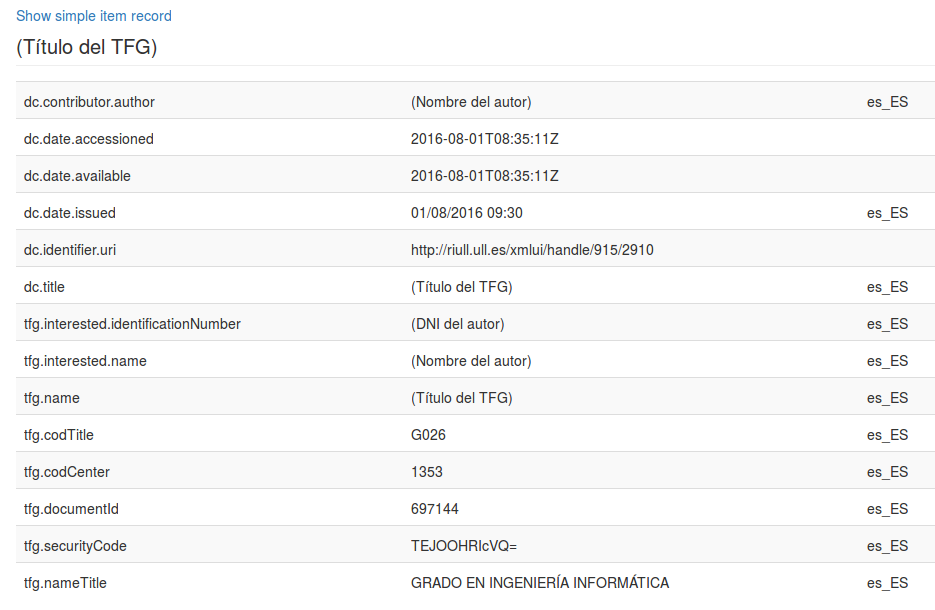
\includegraphics[width=0.8\textwidth]{Images/metadata_view}
\end{figure}
\end{center}

\begin{center}
\begin{minipage}{\linewidth}
\begin{lstlisting}[caption=Función de obtención de metadato por nombre de etiqueta.]
// En una pagina del TFG, obtener el valor del campo 'str' (si lo hay).
function scrapePageValue(str){
    var datum = $('td.label-cell:contains(' + str + ') + td')[0].innerHTML;
    if (datum === null || datum === undefined || datum === "")
        datum = "---";
    return datum;
}
\end{lstlisting}
\end{minipage}
\end{center}

Esta función se basa en la vista de la página para obtener el texto perteneciente a una etiqueta. Por ejemplo, para el caso de la Fig.\ref{fig:metadata_view}, si se le pasa \texttt{author} obtendrá \texttt{(Nombre del autor)}.

% En caso de que no exista, la función devolverá una cadena estándar (en este caso "\texttt{---}") para evitar romper el flujo del programa.

\begin{center}
\begin{minipage}{\linewidth}
\begin{lstlisting}[caption=Función de obtención de metadatos por nombre de etiqueta similar.]
// En una pagina del TFG, obtener el valor de varios campos 'str' (si los hay).
function scrapePageValues(str){
    var data = $('td.label-cell:contains(' + str + ') + td');
    var data2 = [];
    for (var i = 0; i < data.length; i++){
      data2.push(data[i].innerHTML);
    }
    if (data2.length < 1) data2.push("---");
    return data2;
}
\end{lstlisting}
\end{minipage}
\end{center}

Definimos además una función similar a la anterior, con la diferencia de que inspecciona la página para encontrar múltiples datos definidos bajo el mismo nombre. Esto es importante dado que existen metadatos que están definidos bajo campos de mismo nombre, por ejemplo: dos campos de "tema" con distintos valores para expresar que un TFG forma parte de múltiples temas.

\begin{center}
\begin{minipage}{\linewidth}
\begin{lstlisting}[caption=Función de concatenación de enlace.]
function completeLink(currentValue, index, array){
  return 'http://riull.ull.es'.concat(currentValue).concat('?show=full');
}
\end{lstlisting}
\end{minipage}
\end{center}

% Uno de los problemas fue la imposibilidad de realizar una recurrencia sin blabla, por eso se recurrió a crear una función externa

\begin{center}
\begin{minipage}{\linewidth}
\begin{lstlisting}[caption=Función tipo que permite la recurrencia con CasperJS.]
function functionOutsideLoop(){
  links.concat(casper.evaluate(scrapeLinks));
}
\end{lstlisting}
\end{minipage}
\end{center}


%Como primer paso, se le proporciona al navegador CasperJS la página inicial, hacia la cual deberá navegar para iniciar el proceso de extracción. En este caso, es la página que muestra los Trabajos de Fin de Grado para los alumnos del Grado de Informática.

%Una vez en la página de los trabajos de fin de grado, el navegador CasperJS fue programado para obtener los enlaces que le llevarían a las páginas individuales de cada uno de los TFG.

\subsection{Almacenamiento de la información}
\lhead{\emph{\ChapterTwo{}}}
%\subsection{Almacenamiento de la información}
Se decidió guardar la información obtenida del proceso de extracción de texto en archivos locales en el disco duro del ordenador utilizado para la realización del trabajo.

El formato utilizado para los archivos de texto es CSV (\textit{Comma Separated Values}), es decir, archivos de texto planos-
%
Se trata de un formato sencillo en el cual cada elemento se encuentra en una línea diferente, y las características de dichos elementos separados por comas.

La razón por la que se utilizó éste formato se debe a la mayor comodidad que aporta en un caso de estudio restringido, con una cantidad de datos relativamente pequeña.
%
Otra razón por la que se eligió el formato CSV es la disponibilidad de librerías Python que trabajan en este formato, incrementando la facilidad y rapidez de desarrollo del sistema de almacenamiento.

\subsection{Clasificación del texto}
\lhead{\emph{\ChapterFour{}}}

\lstset{
   language=Python
}

\begin{minipage}{\linewidth}
\begin{lstlisting}[caption=Función para cargar instancias de un archivo CSV.]
def cargar_instancias_de_csv(ruta, formato=None):
    """
    Cargamos las instancias de un archivo CSV.

    :param ruta: Ruta del archivo csv que se leerá.
    :param formato: Formato 
    :return: Una lista con cada una de las filas del csv.
    """
    instancias = []
    with open('tfg.csv') as csvfile:
        reader = csv.DictReader(csvfile)
        for row in reader:
            instancias.append((row['Clasificación'], row['Título'], row['Descripción']))
    return instancias
}
\end{lstlisting}
\end{minipage} % Background Theory 

\lhead{\emph{\ChapterThree{}}}
\chaptermark{\emph{\ChapterThree{}}}
\chapter{\ChapterThree{}}
%\lhead{\emph{\ChapterThree{}}}

En este capítulo se expone los resultados alcanzados y se realiza una comparativa entre los métodos utilizados en base a dichos resultados.
%
Además de esto, se destacan los problemas encontrados en las diferentes fases del proceso, y cómo fueron remediados.

\section{Conclusiones sobre la extracción}
La extracción de información fue implementada utilizando selectores de jQuery, para la obtención de los elementos que contienen la información que nos interesa de la vista presente.

Es evidente que este acercamiento es ciertamente inestable, y aumenta la necesidad de mantener el código, debido a que se basa en la jerarquía HTML y estilos CSS de la página que nos es devuelta en una respuesta HTTP. Esta vista puede ser modificada en cualquier momento por los administradores o propietarios de una página web, rompiendo la dependencia y con ella la extracción automatizada. 

En el caso de realizar la extracción de texto en otras páginas web, o incluso la misma página si en un futuro es modificada su vista, deberá modificarse el programa para adaptarse a las nuevas características y disposición que tomen los elementos que contengan la información, siendo esto incómodo y poco óptimo.

Sin embargo, es la única forma de extraer información de una página, servicio, o aplicación web que no disponga de una API (\textit{Application Programming Interface}) que presente la información de manera independiente a la vista o interfaz de usuario.

Otra ventaja del uso de APIs es que evita al interesado descargar la página al completo, de manera que evita descargar archivos pesados que puedan existir en la vista como imágenes, anuncios y etc.

%Esto hace que la implementación de una API también sea preferible para los propietarios de páginas web, porque de la misma manera ahorran el ancho de banda.
%
%Como consecuencia de esto, una API es preferible para los propietarios de las páginas porque evitan consumir su ancho de banda de forma innecesaria, así como para los usuarios de herramientas programáticas por razones anteriormente mencionadas.

%(... creo que habia gente que estaba apostando por una web mas semantica y navegable por maquinas, pero no me lo quiero inventar demasiado...)

A día de hoy, la gran mayoría de páginas y aplicaciones web no poseen una API subyacente, en gran parte debido a la falta de necesidad que se tiene de ello, ya que no están pensadas para obtener la información mediante métodos programáticos.

Es ideal que todo servicio o página web disponga de una API como punto de entrada de datos a una aplicación, pero en su defecto también es factible que en la vista se realice un etiquetado semántico de los elementos, ya sea mediante HTML o CSS, proporcionando cierta autonomía de la vista de la página.

A pesar de esto, en la mayoría de los casos los administradores y propietarios de las páginas web no tienen incentivos ni necesidad de suplir esta necesidad, por lo que se deberá seguir utilizando estas técnicas de extracción de datos o \textit{web scraping}.

\section{Conclusiones sobre la clasificaión}
\lhead{\emph{\ChapterThree{}}}
\label{classification-conclusions}
El primer acercamiento de clasificación se realizó utilizando los metadatos disponibles para cada uno de los TFGs, concretamente el título y el abstracto. Se utilizó el campo de "tema" para determinar la clasificación que se le había dado a cada TFG en el RIULL.
%

Se realizó una batería de pruebas, variando el número de palabras comunes a considerar. Se empezó utilizando las 100 palabras más comunes, aumentando esto en incrementos de 100 hasta llegar a un clasificador que considera las 2000 palabras más comunes entre los textos a clasificar.

\begin{center}
\begin{figure}[!ht]
  \label{fig:metadata_view}
  \centering
    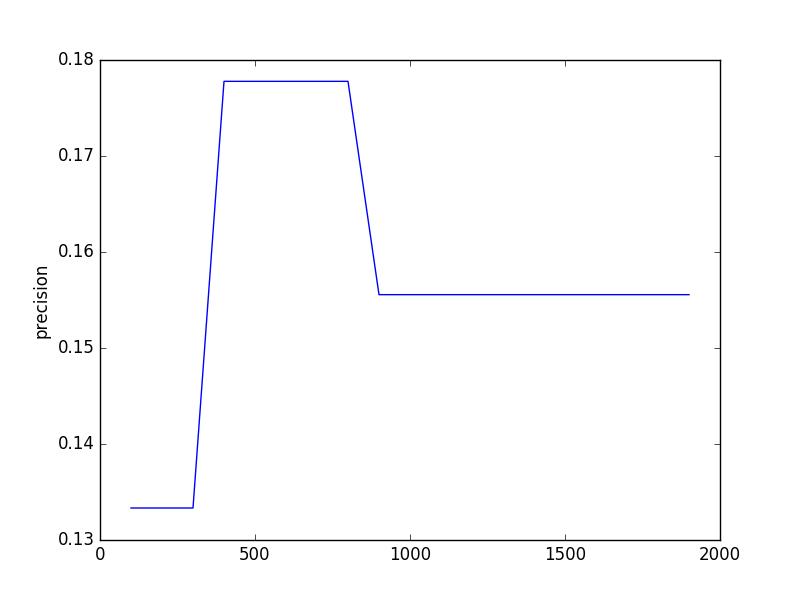
\includegraphics[width=0.8\textwidth]{Images/figure_1}
  \caption{Precisión de la clasificación Naive Bayes usando metadatos de los TFG de Ing. Informática.}
\end{figure}
\end{center}

Como vemos, la precisión del clasificador oscila entre 0.13 y 0.18, lo que indica que el clasificador acierta entre el 13\% y 18\% de las veces. Estos resultados son bastante pobres, y esto se debe a la poca información que proporcionan los metadatos existentes sobre los textos.
%
La falta de información se debe a tres factores: en primer lugar, los títulos no suelen sobrepasar las 20 palabras, lo que hace difícil la clasificación por conteo de palabras comunes. 
%
El segundo problema es que en muchos casos, la descripción o abstracto del TFG no se encuentra como metadato del TFG en la RIULL, debido a ser un campo opcional.
%
Finalmente, se tiene un número elevado de clases, muchas de ellas conteniendo a un único TFG, lo que reduce las posibilidades de caracterizar una clase y aumenta las probabilidades de cometer una asignación errónea.

Por otra parte, podemos observar cómo decrementa la precisión del clasificador a partir de un número de palabras dado. Podemos inducir de esto que existe un límite de palabras a considerar óptimo, tras el cual se consideran demasiadas características de los elementos como para dar una respuesta fiable.

\section{Problemas encontrados}
\lhead{\emph{\ChapterThree{}}}
\subsection{Obtención del texto}

Uno de los problemas a la hora de realizar la extracción de texto en la página del Repositorio Institucional de la ULL se producía cuando se realizaba un número excesivo de consultas a la página. Esto provocaba que las peticiones enviadas desde la IP del ordenador de pruebas fuesen ignoradas por el servidor. Se puede conjeturar que esto sea resultado de un mecanismo de defensa del servidor institucional para contrarrestar ataques DoS (\textit{Denial of Service}). 
\todo{
Esto provocaba una interrupción en el flujo de trabajo, impidiendo la obtención de datos hasta 
}

\subsection{Clasificación del texto}

% Para la clasificación de los textos DURANTE LA PRIMERA APROXIMACION
Para la clasificación de los textos, uno de los problemas más importantes fue el exceso de clases en comparación con el número de instancias. Muchas de estas clases contenían a un único elemento, lo que dificultaba el proceso de clasificación al no obtener suficiente información determinante para caracterizar cada tipo de clase.

Como se comentó en el apartado \ref{classification-conclusions}, en muchos casos, la descripción o abstracto del TFG no se encuentra como metadato de los TFG de la RIULL, debido a que no es obligatorio rellenar este campo para dar de alta un TFG en la plataforma.
%
Esto redujo drásticamente la capacidad de clasificación sobre los metadatos de los TFGs en comparación con el caso en que todos los documentos tuviesen un resumen o abstracto asignado en el servicio.

Las bajas tasas de acierto resultan poco alentadoras, pero se deben a la presencia de clases con pocas entidades representativas, así como la falta de información individual sobre cada TFG en forma de metadatos. Esto se puede paliar ignorando las clases que no posean un número mínimo de instancias, centrándonos en clasificar aquéllas clases que podamos caracterizar correctamente gracias a su número elevado de integrantes. 
%
La otra solución es la obtención de más información característica sobre cada instancia individual, lo que se consigue extrayendo información textual de los documentos infijos (extensión PDF) aparte de sus metadatos.

\subsection{Realización de la memoria}

Por defecto \textit{LaTeX} no permite el uso de tildes y caracteres españoles, por lo que fue necesario incluir el paquete \texttt{inputenc} y \texttt{babel} en la configuración del proyecto, con las opciones \texttt{utf8} y \texttt{spanish}, respectivamente.

A la hora de mostrar el código del trabajo realizado, el primer método considerado fue la realización de capturas del código en el editor de texto, para insertarlas en el documento como imágenes.
Esto conllevaba una falta de uniformidad, debido al diferente tamaño de las imágenes, así como dificultad a la hora de cambiar la apariencia de las mismas.

Como alternativa, se utilizó un paquete \textit{LaTeX} llamado \texttt{listings}, que permite la introducción de código con formato, y proporciona funcionalidad que ayuda a su lectura como el resaltado (\textit{highlighting}) de palabras reservadas.
%
Tuvo que ser modificado para permitir el resaltado de código JavaScript, cuya sintaxis no se incluía por defecto, para resaltar los listados apropiados. % Experimental Setup

\lhead{\emph{\ChapterFour{}}}
\chaptermark{\emph{\ChapterFour{}}}
\chapter{\ChapterFour{}}
%\lhead{\emph{\ChapterFour{}}}

\section{Conclusiones y Trabajos Futuros}

Como líneas futuras de trabajo, se considera la extracción de texto de los Trabajos de Fin de Grado en formato infijo (extensión PDF), con el fin de obtener una cantidad suficiente de palabras para caracterizar cada una de las instancias a clasificar.

Por otra parte, se tiene en cuenta la posibilidad de descargar datos de TFGs de diferentes disciplinas a la Informática, para aumentar la diferenciación entre instancias y esperando que la capacidad de clasificación incremente de manera considerable.

Finalmente, se puede utilizar un clasificador estadístico diferente al clasificador bayesiano ingenuo, o también considerar otros métodos de definición y extracción de características.

---

Las técnicas de Procesamiento del Lenguaje Natural tienen hoy en día un gran número de aplicaciones prácticas, gracias a la disponibilidad de una gran cantidad de datos en Internet y a la creciente capacidad de procesamiento tradicional y en la nube (\textit{cloud computing}), dando soporte a las técnicas de aprendizaje estadístico que gozan de gran aceptación en la actualidad.

La herramienta que goza de mayor popularidad actualmente tanto para el Procesamiento del Lenguaje Natural como otras ramas de la Computación es el Aprendizaje Automático, gracias a la mayor cantidad de información y capacidad de procesamiento disponibles.

Esta herramienta ha permitido un incremento considerable de las aplicaciones prácticas del Procesamiento del Lenguaje Natural durante la última década. Esto ha creado nuevos puestos de trabajo en grandes compañías y pequeñas \textit{startups} de nueva creación que han decidido tomar la oportunidad que estas nuevas tecnologías brindan.

Esta inversión en el área del Procesamiento del Lenguaje Natural también se ve reflejada en el ámbito académico, y producirá durante las próximas décadas nuevas herramientas y aplicaciones para la sociedad, en sinergia con los campos de la Interacción Persona-Computador y la Inteligencia Artificial.

\section{Conclusions and Future Work}

For future lines of work, we will consider the extraction of the Final Degree Projects in infix format (PDF extension), in order to obtain a sufficient amount of words so as to characterize each of the instances that are to be classified.

We also take into account the possibility of downloading data from Final Degree Projects of fields different from Computer Science, in order to increase the differentiation between instances and in hopes of increasing the classification capacity considerably.

Finally, a classifier different from the Naive Bayes classifier can be used, or different methods of feature definition and extraction can be considered.

---

At present, Natural Language Processing techniques have a wide range of practical applications, thanks to the availability of a vast amount of data on the Internet and the increasing processing capabilities of computers, both locally and in cloud computing, supporting the statistical learning techniques that are widely accepted to date.

The tool which has garnered the most popularity in recent years, in the field of Natural Language Processing as well as other fields of Computer Science, is Machine Learning, thanks to the higher amount of information and computational power currently available.

This tool has allowed for a significant increase of the practical applications of Natural Language Processing during the last decade. This has created new jobs in large companies and newly-created \textit{startups} that have seized the opportunity that these new technologies bring.

This investment in the area of Natural Language Processing is also reflected in the academical world, and in the next decades it will provide new tools and applications for society, in synergy with the fields of Human-Computer Interaction and Artificial Intelligence. % Experiment 1

\lhead{\emph{\ChapterFive{}}}
\chaptermark{\emph{\ChapterFive{}}}
\chapter{\ChapterFive{}}
\lhead{\emph{\ChapterFive{}}}

\setstretch{1.5}  % Set the line spacing to 1.5, this makes the following tables easier to read

\begin{table}[!ht]
\centering
\caption{Presupuesto}
\label{tabla-presupuesto}
\begin{tabular}{|l|l|l|l|}
\hline
Descripción      & Costo por unidad & Cantidad & Costo total \\ \hline
Horas de trabajo & 9\euro{}         & 300      & 2700\euro{} \\ \hline
Total:           & ---              & ---      & 2700\euro{} \\ \hline
\end{tabular}
\end{table} % Experiment 2

%% ----------------------------------------------------------------
% Now begin the Appendices, including them as separate files

\addtocontents{toc}{\vspace{2em}} % Add a gap in the Contents, for aesthetics

\appendix % Cue to tell LaTeX that the following 'chapters' are Appendices

\lhead{\emph{Abbreviations}}  % Set the left side page header to "Abbreviations"
\chapter{Abreviaturas}
\begin{itemize}
    \item \textbf{API}: \textit{\textbf{A}pplication \textbf{P}rogramming \textbf{I}nterface}
    \item \textbf{CSS}: \textit{\textbf{C}ascading \textbf{S}tyle \textbf{S}heets}
    \item \textbf{CSV}: \textit{\textbf{C}omma \textbf{S}eparated \textbf{V}alues}
    \item \textbf{DOM}: \textit{\textbf{D}ocument \textbf{O}bject \textbf{M}odel}
    \item \textbf{HTML}: \textit{\textbf{H}yper\textbf{T}ext  \textbf{M}arkup \textbf{L}anguage}
    \item \textbf{HTTP}: \textit{\textbf{H}yper\textbf{T}ext  \textbf{T}ransfer \textbf{P}rotocol}
    \item \textbf{NLTK}: \textit{\textbf{N}atural \textbf{L}anguage \textbf{T}ool\textbf{K}it}
    \item \textbf{PDF}: \textit{\textbf{P}ortable \textbf{D}ocument \textbf{F}ormat}
    \item \textbf{PLN}: \textbf{P}rocesamiento del \textbf{L}enguaje \textbf{N}atural
    \item \textbf{RIULL}: \textbf{R}epositorio \textbf{I}nstitucional de la \textbf{U}niversidad de \textbf{L}a \textbf{L}aguna
    \item \textbf{TFG}: \textbf{T}rabajo de \textbf{F}in de \textbf{G}rado
\end{itemize}	% Abreviaturas

%\pagestyle{empty}  % Page style needs to be empty for this page

\lhead{\emph{Glosario}}  % Set the left side page header to "Abbreviations"
\chapter{Glosario}

\textbf{API:} \textit{Application Programming Interface}, interfaz que permite la interacción con un sistema informático de manera programática mediante código, sin necesidad de interactuar de forma manual a través de una interfaz de usuario.

\textbf{Metadatos:} Datos que acompañan a un archivo o documento informático, contextualizando su creación y denotando sus características, sin llegar a formar parte del contenido del documento en sí.

\textbf{\textit{Parser:}} Programa que recibe información de manera secuencial y tiene como cometido desglosar la información que se le pasa como entrada en datos estructurados en la memoria de un sistema.

\textbf{\textit{Web scraping:}} Procedimiento mediante el cual se obtiene información de una página web, obteniéndose a través del protocolo HTTP, y luego extrayendo la información relevante mediante expresiones regulares o \textit{parsers} de DOM o HTML. % Glosario

%\input{Appendices/AppendixC} % Appendix Title

\addtocontents{toc}{\vspace{2em}}  % Add a gap in the Contents, for aesthetics
\backmatter

%% ----------------------------------------------------------------
%\label{Bibliography}
%\lhead{\emph{Bibliography}}  % Change the left side page header to "Bibliography"
%\bibliographystyle{unsrtnat}  % Use the "unsrtnat" BibTeX style for formatting the Bibliography
%\bibliography{Bibliography}  % The references (bibliography) information are stored in the file named "Bibliography.bib"

%\begin{thebibliography}{9}

%\bibitem{lamport94}
%  Leslie Lamport,
%  \emph{\LaTeX: a document preparation system},
%  Addison Wesley, Massachusetts,
%  2nd edition,
%  1994.
  
\bibitem{bird09}
  Steven Bird, Ewan Klein, Edward Loper,
  \emph{Natural Language Processing With Python},
  %Url = {http://www.nltk.org/book/},
  2009.

\bibitem{gate}
  GATE,
  \emph{General Architecture for Text Engineering},
  https://gate.ac.uk/
  
\bibitem{gate_about}
  GATE,
  \emph{The GATE Project Team},
  https://gate.ac.uk/people/

\bibitem{epsrc}
  Engineering and Physical Sciences Research Council,
  \emph{EPSRC Webpage},
  https://www.epsrc.ac.uk/

\bibitem{sepln}
  Sociedad Española para el Procesamiento del Lenguaje Natural,
  \emph{Página principal},
  http://www.sepln.org/,
  2016.

\bibitem{sepln-56}
  Sociedad Española para el Procesamiento del Lenguaje Natural,
  \emph{Revista SEPLN nº56},
  http://www.sepln.org/news/revista-nº-56/,
  2016.
  
\bibitem{casper-js}
  CasperJS Team,
  \emph{CasperJS, a navigation scripting and testing utility for PhantomJS and SlimerJS},
  casperjs.org,
  2011.
\end{thebibliography}
\bibliographystyle{plain}
\bibliography{Bibliography} 

\end{document}  % The End
%% ----------------------------------------------------------------